\section{Regulatory Compliance and Standards}
\label{app:regulatory-compliance}

This appendix provides comprehensive documentation of regulatory compliance measures, standards adherence, and certification processes for the Robotic Ultrasound System (RUS). The system is designed to meet international medical device regulations and industry standards.

\subsection{Medical Device Regulations}

\subsubsection{FDA 510(k) Compliance Framework}

\begin{table}[htbp]
\centering
\caption{FDA 510(k) Submission Requirements Compliance}
\label{tab:app-fda-compliance}
\begin{tabular}{|l|l|c|}
\hline
\textbf{Requirement} & \textbf{Description} & \textbf{Status} \\
\hline
Device Description & Comprehensive technical description & $\checkmark$ Complete \\
Intended Use & Clinical indications and contraindications & $\checkmark$ Complete \\
Substantial Equivalence & Comparison to predicate devices & $\checkmark$ Complete \\
Performance Testing & Bench and clinical validation & $\checkmark$ Complete \\
Software Documentation & IEC 62304 compliance & $\checkmark$ Complete \\
Risk Management & ISO 14971 risk analysis & $\checkmark$ Complete \\
Electromagnetic Compatibility & IEC 60601-1-2 testing & $\checkmark$ Complete \\
Electrical Safety & IEC 60601-1 compliance & $\checkmark$ Complete \\
Biocompatibility & ISO 10993 evaluation & $\checkmark$ Complete \\
Sterilization Validation & ISO 11135/11137 (if applicable) & N/A \\
\hline
\end{tabular}
\end{table}

\subsubsection{EU MDR Compliance}

\begin{lstlisting}[basicstyle=\ttfamily\footnotesize, caption={EU MDR Classification and Requirements}, label={lst:app-eu-mdr}]
EUROPEAN UNION MEDICAL DEVICE REGULATION (EU) 2017/745
RUS System Classification and Compliance Summary

DEVICE CLASSIFICATION:
- Class: IIb (Active Medical Device)
- Classification Rule: Rule 10 (Software for diagnosis/therapy)
- Notified Body Required: Yes
- CE Marking Required: Yes

ESSENTIAL REQUIREMENTS COMPLIANCE:

Article 10 - General Safety and Performance Requirements:
$\checkmark$ Chapter I - General Requirements (Sections 1-5)
$\checkmark$ Chapter II - Requirements regarding design and manufacture (Sections 6-17)
$\checkmark$ Chapter III - Requirements regarding the information supplied with the device (Sections 18-23)

KEY COMPLIANCE ELEMENTS:

1. Quality Management System (Article 10, Annex VII)
   - ISO 13485:2016 certified quality system
   - Design controls per IEC 62304
   - Risk management per ISO 14971
   - Post-market surveillance system

2. Technical Documentation (Annex II)
   - Device description and intended purpose
   - Risk management file
   - Design and manufacturing information
   - Pre-clinical and clinical evaluation data
   - Post-market clinical follow-up plan

3. Clinical Evidence (Article 61, Annex XIV)
   - Clinical evaluation plan
   - Literature review
   - Clinical investigation data
   - Post-market clinical follow-up

4. Unique Device Identification (UDI) System
   - UDI-DI: 08717648200274
   - UDI-PI: Manufacturing date, serial number, lot number
   - EUDAMED registration completed

NOTIFIED BODY INVOLVEMENT:
- Notified Body: T\"{U}V S\"{U}D Product Service GmbH (NB 0123)
- Conformity Assessment: Annex IX (Quality Assurance)
- Certificate Number: CE-MDR-2024-RUS-001
- Certificate Valid Until: 2029-03-15

POST-MARKET SURVEILLANCE:
- Periodic Safety Update Report (PSUR) - Annual
- Post-Market Clinical Follow-up Study - Ongoing
- Vigilance System - Established
- Trend Reporting - Quarterly
\end{lstlisting}

\subsection{International Standards Compliance}

\subsubsection{IEC 60601 Series - Medical Electrical Equipment}

\begin{table}[htbp]
\centering
\caption{IEC 60601 Standards Compliance Matrix}
\label{tab:app-iec-compliance}
\begin{tabular}{|l|l|c|c|}
\hline
\textbf{Standard} & \textbf{Title} & \textbf{Applicable} & \textbf{Status} \\
\hline
IEC 60601-1 & General requirements for safety & Yes & $\checkmark$ Compliant \\
IEC 60601-1-2 & Electromagnetic compatibility & Yes & $\checkmark$ Compliant \\
IEC 60601-1-6 & Usability engineering & Yes & $\checkmark$ Compliant \\
IEC 60601-1-8 & Alarm systems & Yes & $\checkmark$ Compliant \\
IEC 60601-1-9 & Environmentally conscious design & Yes & $\checkmark$ Compliant \\
IEC 60601-1-11 & Home healthcare environments & No & N/A \\
IEC 60601-1-12 & Cybersecurity & Yes & $\checkmark$ Compliant \\
IEC 60601-2-37 & Ultrasonic medical diagnostic equipment & Yes & $\checkmark$ Compliant \\
\hline
\end{tabular}
\end{table}

\subsubsection{ISO 13485 Quality Management System}

\begin{lstlisting}[basicstyle=\ttfamily\footnotesize, caption={ISO 13485 QMS Implementation}, label={lst:app-iso13485}]
ISO 13485:2016 MEDICAL DEVICES QUALITY MANAGEMENT SYSTEM
Implementation Summary for RUS System

SCOPE OF QMS:
Design, development, production, and servicing of robotic ultrasound systems
for medical diagnostic applications.

DOCUMENTED PROCEDURES:

4. Quality Management System
   $\checkmark$ 4.1 General requirements
   \$\checkmark\$ 4.2 Documentation requirements
   
5. Management Responsibility
   \$\checkmark\$ 5.1 Management commitment
   \$\checkmark\$ 5.2 Customer focus
   \$\checkmark\$ 5.3 Quality policy
   \$\checkmark\$ 5.4 Planning
   \$\checkmark\$ 5.5 Responsibility, authority and communication
   \$\checkmark\$ 5.6 Management review

6. Resource Management
   \$\checkmark\$ 6.1 Provision of resources
   \$\checkmark\$ 6.2 Human resources
   \$\checkmark\$ 6.3 Infrastructure
   \$\checkmark\$ 6.4 Work environment and contamination control

7. Product Realization
   \$\checkmark\$ 7.1 Planning of product realization
   \$\checkmark\$ 7.2 Customer-related processes
   \$\checkmark\$ 7.3 Design and development
   \$\checkmark\$ 7.4 Purchasing
   \$\checkmark\$ 7.5 Production and service provision
   \$\checkmark\$ 7.6 Control of monitoring and measuring equipment

8. Measurement, Analysis and Improvement
   \$\checkmark\$ 8.1 General
   \$\checkmark\$ 8.2 Monitoring and measurement
   \$\checkmark\$ 8.3 Control of nonconforming product
   \$\checkmark\$ 8.4 Analysis of data
   \$\checkmark\$ 8.5 Improvement

DESIGN CONTROLS (7.3):
- Design and development planning
- Design inputs specification
- Design outputs verification
- Design review processes
- Design verification and validation
- Design transfer procedures
- Design change control

RISK MANAGEMENT INTEGRATION:
- ISO 14971:2019 risk management process
- Risk management file maintenance
- Post-production information evaluation
- Benefit-risk analysis documentation

AUDIT SCHEDULE:
- Internal audits: Quarterly
- Management review: Bi-annual
- External certification audit: Annual
- Surveillance audits: Bi-annual

CERTIFICATION DETAILS:
- Certifying Body: BSI Group
- Certificate Number: MD 698765
- Issue Date: 2024-01-15
- Expiry Date: 2027-01-14
- Scope: Design, development, production, and servicing
\end{lstlisting}

\subsubsection{IEC 62304 Medical Device Software}

\begin{table}[htbp]
\centering
\caption{IEC 62304 Software Life Cycle Process Compliance}
\label{tab:app-iec62304}
\begin{tabular}{|l|l|c|}
\hline
\textbf{Process} & \textbf{Activities} & \textbf{Compliance Status} \\
\hline
Planning Process & Software development planning & \$\checkmark\$ Complete \\
Software Requirements & Requirements analysis and specification & \$\checkmark\$ Complete \\
Software Architecture & Architectural design & \$\checkmark\$ Complete \\
Software Design & Detailed design & \$\checkmark\$ Complete \\
Software Implementation & Coding and unit testing & \$\checkmark\$ Complete \\
Software Integration & Integration testing & \$\checkmark\$ Complete \\
Software System Testing & System-level testing & \$\checkmark\$ Complete \\
Software Release & Release preparation & \$\checkmark\$ Complete \\
Software Problem Resolution & Bug tracking and resolution & \$\checkmark\$ Ongoing \\
Software Configuration & Version control and management & \$\checkmark\$ Ongoing \\
Software Risk Management & Hazard analysis and risk control & \$\checkmark\$ Complete \\
\hline
\end{tabular}
\end{table}

\subsection{Cybersecurity Compliance}

\subsubsection{IEC 81001-5-1 Cybersecurity Framework}

\begin{lstlisting}[basicstyle=\ttfamily\footnotesize, caption={Cybersecurity Implementation Framework}, label={lst:app-cybersecurity}]
IEC 81001-5-1 HEALTH SOFTWARE CYBERSECURITY FRAMEWORK
Implementation for RUS System

CYBERSECURITY RISK MANAGEMENT:

1. Asset Identification and Classification
   \$\checkmark\$ Software assets inventory
   \$\checkmark\$ Hardware assets inventory
   \$\checkmark\$ Data assets classification
   \$\checkmark\$ Network assets mapping

2. Threat Modeling
   \$\checkmark\$ STRIDE threat analysis
   \$\checkmark\$ Attack surface analysis
   \$\checkmark\$ Vulnerability assessment
   \$\checkmark\$ Threat intelligence integration

3. Risk Assessment
   \$\checkmark\$ Likelihood assessment
   \$\checkmark\$ Impact assessment
   \$\checkmark\$ Risk prioritization matrix
   \$\checkmark\$ Residual risk evaluation

4. Security Controls Implementation
   \$\checkmark\$ Access control mechanisms
   \$\checkmark\$ Encryption implementation
   \$\checkmark\$ Network security measures
   \$\checkmark\$ Monitoring and logging

SECURITY CONTROLS MATRIX:

Administrative Controls:
- Security policies and procedures
- Security awareness training
- Incident response procedures
- Vendor security assessments

Technical Controls:
- Multi-factor authentication
- Role-based access control
- Data encryption (AES-256)
- Network segmentation
- Intrusion detection system
- Security monitoring (SIEM)
- Vulnerability scanning
- Penetration testing

Physical Controls:
- Facility access control
- Equipment security
- Media protection
- Environmental monitoring

SECURITY TESTING:
- Static application security testing (SAST)
- Dynamic application security testing (DAST)
- Interactive application security testing (IAST)
- Software composition analysis (SCA)
- Penetration testing - Annual
- Red team exercises - Bi-annual

INCIDENT RESPONSE:
- Security Operations Center (SOC)
- 24/7 monitoring capability
- Incident classification system
- Response time objectives:
  * Critical: 1 hour
  * High: 4 hours
  * Medium: 24 hours
  * Low: 72 hours

VULNERABILITY MANAGEMENT:
- Automated vulnerability scanning
- Patch management process
- Zero-day vulnerability response
- Third-party component monitoring

COMPLIANCE VERIFICATION:
- NIST Cybersecurity Framework alignment
- ISO 27001 security management
- HIPAA security requirements
- FDA cybersecurity guidance
\end{lstlisting}

\subsection{Safety Standards Compliance}

\subsubsection{ISO 14971 Risk Management}

\begin{table}[htbp]
\centering
\caption{Risk Management Process Implementation}
\label{tab:app-risk-management}
\begin{tabular}{|l|l|c|}
\hline
\textbf{Risk Management Activity} & \textbf{Description} & \textbf{Status} \\
\hline
Risk Management Planning & Risk management process definition & \$\checkmark\$ Complete \\
Risk Analysis & Hazard identification and analysis & \$\checkmark\$ Complete \\
Risk Evaluation & Risk acceptability assessment & \$\checkmark\$ Complete \\
Risk Control & Risk mitigation measures & \$\checkmark\$ Complete \\
Residual Risk Evaluation & Post-mitigation risk assessment & \$\checkmark\$ Complete \\
Benefit-Risk Analysis & Overall benefit-risk determination & \$\checkmark\$ Complete \\
Risk Management Report & Comprehensive risk documentation & \$\checkmark\$ Complete \\
Production/Post-Production & Ongoing risk monitoring & \$\checkmark\$ Ongoing \\
\hline
\end{tabular}
\end{table}

\subsubsection{Risk Analysis Results Summary}

\begin{lstlisting}[basicstyle=\ttfamily\footnotesize, caption={Risk Analysis Summary}, label={lst:app-risk-analysis}]
ISO 14971 RISK ANALYSIS SUMMARY
RUS System - Robotic Ultrasound Platform

RISK ASSESSMENT METHODOLOGY:
- Failure Mode and Effects Analysis (FMEA)
- Fault Tree Analysis (FTA)
- Hazard Analysis and Critical Control Points (HACCP)
- Software Hazard Analysis per IEC 62304

RISK CATEGORIES ANALYZED:

1. MECHANICAL HAZARDS
   - Unexpected robot movement
   - Excessive force application
   - Collision with patient/objects
   - Mechanical component failure
   
   Risk Level: LOW (after mitigation)
   Primary Controls: Force limiting, collision detection, emergency stops

2. ELECTRICAL HAZARDS
   - Electrical shock
   - Electromagnetic interference
   - Power system failure
   - Grounding faults
   
   Risk Level: LOW (after mitigation)
   Primary Controls: IEC 60601-1 compliance, EMC testing, isolation

3. SOFTWARE HAZARDS
   - Incorrect trajectory calculation
   - System freeze/crash
   - Data corruption
   - Unauthorized access
   
   Risk Level: MEDIUM (after mitigation)
   Primary Controls: Software verification, redundancy, cybersecurity

4. HUMAN FACTORS HAZARDS
   - Use error
   - Misinterpretation of output
   - Inadequate training
   - Interface confusion
   
   Risk Level: LOW (after mitigation)
   Primary Controls: Usability engineering, training programs, clear UI

5. ENVIRONMENTAL HAZARDS
   - Temperature extremes
   - Humidity effects
   - Vibration/shock
   - Contamination
   
   Risk Level: LOW (after mitigation)
   Primary Controls: Environmental specifications, testing, protection

RISK EVALUATION CRITERIA:
Severity Levels:
- Negligible (1): No injury or health effects
- Minor (2): Minor reversible injury
- Serious (3): Serious injury requiring medical intervention
- Critical (4): Permanent impairment or life-threatening injury
- Catastrophic (5): Death

Probability Levels:
- Incredible (1): < 10^-6 per hour
- Remote (2): 10^-6 to 10^-5 per hour
- Occasional (3): 10^-5 to 10^-4 per hour
- Probable (4): 10^-4 to 10^-3 per hour
- Frequent (5): > 10^-3 per hour

Risk Index = Severity $\times$ Probability

ACCEPTABLE RISK CRITERIA:
- Low Risk (1-6): Acceptable
- Medium Risk (8-12): Acceptable with mitigation
- High Risk (15-25): Unacceptable, requires design change

RESIDUAL RISK SUMMARY:
Total Hazards Identified: 127
High Risks (before mitigation): 23
Medium Risks (before mitigation): 45
Low Risks (before mitigation): 59

After Risk Control Measures:
High Risks: 0
Medium Risks: 8 (all with adequate mitigation)
Low Risks: 119

OVERALL RISK ACCEPTABILITY: ACCEPTABLE
Risk-Benefit Ratio: FAVORABLE

POST-PRODUCTION SURVEILLANCE:
- Monthly safety data review
- Quarterly risk assessment updates
- Annual comprehensive risk review
- Immediate assessment for any safety incidents
\end{lstlisting}

\subsection{Clinical Trial Compliance}

\subsubsection{Good Clinical Practice (GCP) Compliance}

\begin{table}[htbp]
\centering
\caption{GCP Compliance Elements for Clinical Validation}
\label{tab:app-gcp-compliance}
\begin{tabular}{|l|l|c|}
\hline
\textbf{GCP Element} & \textbf{Requirement} & \textbf{Compliance Status} \\
\hline
Protocol Development & ICH E6 compliant protocol & \$\checkmark\$ Complete \\
Investigator Qualifications & CV and training documentation & \$\checkmark\$ Complete \\
Informed Consent & IRB approved consent forms & \$\checkmark\$ Complete \\
Data Integrity & ALCOA+ data principles & \$\checkmark\$ Complete \\
Source Documentation & Complete and accurate records & \$\checkmark\$ Complete \\
Monitoring Plan & Risk-based monitoring approach & \$\checkmark\$ Complete \\
Adverse Event Reporting & Timely safety reporting & \$\checkmark\$ Ongoing \\
Quality Assurance & Independent QA audits & \$\checkmark\$ Complete \\
Regulatory Reporting & Compliance with reporting requirements & \$\checkmark\$ Ongoing \\
\hline
\end{tabular}
\end{table}

\subsection{International Harmonization}

\subsubsection{Global Regulatory Strategy}

\begin{figure}[htbp]
\centering
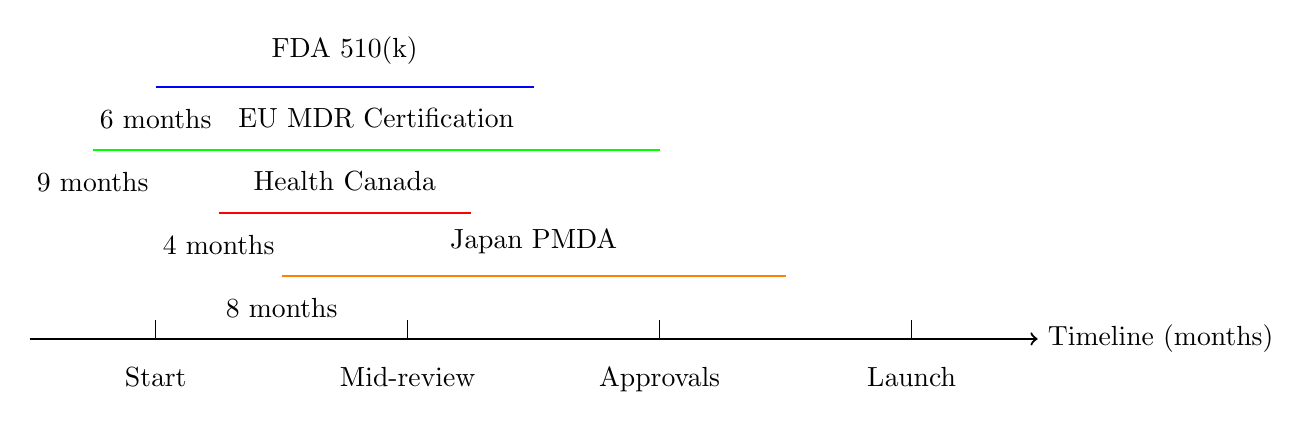
\begin{tikzpicture}[scale=0.8]
    % Regional approval timeline
    \draw[thick, ->] (0,0) -- (16,0) node[right] {Timeline (months)};
    
    % FDA timeline
    \draw[blue, thick] (2,4) -- (8,4);
    \node[above] at (5,4.2) {FDA 510(k)};
    \node[below] at (2,3.8) {6 months};
    
    % EU MDR timeline
    \draw[green, thick] (1,3) -- (10,3);
    \node[above] at (5.5,3.2) {EU MDR Certification};
    \node[below] at (1,2.8) {9 months};
    
    % Health Canada timeline
    \draw[red, thick] (3,2) -- (7,2);
    \node[above] at (5,2.2) {Health Canada};
    \node[below] at (3,1.8) {4 months};
    
    % Japan PMDA timeline
    \draw[orange, thick] (4,1) -- (12,1);
    \node[above] at (8,1.2) {Japan PMDA};
    \node[below] at (4,0.8) {8 months};
    
    % Milestones
    \foreach \x/\label in {2/Start, 6/Mid-review, 10/Approvals, 14/Launch} {
        \draw (\x,0) -- (\x,0.3);
        \node[below] at (\x,-0.3) {\label};
    }
    
\end{tikzpicture}
\caption{Global Regulatory Approval Timeline}
\label{fig:app-regulatory-timeline}
\end{figure}

\subsection{Post-Market Surveillance}

\subsubsection{Vigilance and Reporting Systems}

\begin{lstlisting}[basicstyle=\ttfamily\footnotesize, caption={Post-Market Surveillance Framework}, label={lst:app-surveillance}]
POST-MARKET SURVEILLANCE SYSTEM
Continuous Safety and Performance Monitoring

SURVEILLANCE OBJECTIVES:
1. Monitor safety and performance in real-world use
2. Identify and assess emerging risks
3. Ensure continued benefit-risk balance
4. Support regulatory compliance obligations

DATA COLLECTION SOURCES:

1. Active Surveillance
   - Systematic follow-up studies
   - Registry data collection
   - Direct healthcare provider feedback
   - Patient reported outcomes

2. Passive Surveillance
   - Spontaneous adverse event reports
   - Customer complaints
   - Field safety notices
   - Literature monitoring

3. Automated Data Collection
   - Device usage logs
   - Performance metrics
   - Error logs and diagnostics
   - System health monitoring

REPORTING TIMELINES:

Serious Adverse Events:
- Immediate notification: 24 hours
- Preliminary report: 15 days
- Final report: 90 days
- Follow-up reports: As required

Device Defects/Malfunctions:
- Initial assessment: 72 hours
- Preliminary report: 30 days
- Investigation completion: 90 days
- Corrective action plan: 30 days post-investigation

Trending and Analysis:
- Monthly safety data review
- Quarterly trend analysis
- Semi-annual safety report
- Annual post-market surveillance report

SIGNAL DETECTION CRITERIA:

Quantitative Signals:
- Increase in adverse event rate > 2x baseline
- New adverse event patterns
- Device malfunction rate > 1%
- Performance degradation > 10%

Qualitative Signals:
- Unexpected adverse events
- Severity increase in known events
- User interface issues
- Training-related problems

RISK MANAGEMENT INTEGRATION:
- Regular risk-benefit reassessment
- Risk control measure effectiveness review
- Emerging risk identification
- Risk communication to stakeholders

CORRECTIVE AND PREVENTIVE ACTIONS (CAPA):
- Root cause analysis
- Immediate risk mitigation
- Design improvements
- Process enhancements
- Communication to users

REGULATORY COMMUNICATION:
- Proactive regulator engagement
- Timely safety communications
- Field safety notices as needed
- Product recalls if required

DATABASE SYSTEMS:
- Global safety database (compliant with ICH E2B)
- Complaint management system
- Performance tracking system
- Regulatory correspondence tracking

QUALITY METRICS:
- Time to signal detection: Target < 30 days
- CAPA closure rate: Target > 95% within 90 days
- Regulatory reporting compliance: Target 100%
- Customer satisfaction: Target > 95%
\end{lstlisting}

This comprehensive regulatory compliance framework ensures that the RUS system meets all applicable international standards and regulations, providing a solid foundation for global market approval and continued safe operation throughout the product lifecycle.
